%DIF PREAMBLE EXTENSION ADDED BY LATEXDIFF
%DIF UNDERLINE PREAMBLE %DIF PREAMBLE
\RequirePackage[normalem]{ulem} %DIF PREAMBLE
\RequirePackage{color}\definecolor{RED}{rgb}{1,0,0}\definecolor{BLUE}{rgb}{0,0,1} %DIF PREAMBLE
\providecommand{\DIFadd}[1]{{\protect\color{blue}\uwave{#1}}} %DIF PREAMBLE
\providecommand{\DIFdel}[1]{{\protect\color{red}\sout{#1}}} %DIF PREAMBLE
%DIF SAFE PREAMBLE %DIF PREAMBLE
\providecommand{\DIFaddbegin}{} %DIF PREAMBLE
\providecommand{\DIFaddend}{} %DIF PREAMBLE
\providecommand{\DIFdelbegin}{} %DIF PREAMBLE
\providecommand{\DIFdelend}{} %DIF PREAMBLE
%DIF FLOATSAFE PREAMBLE %DIF PREAMBLE
\providecommand{\DIFaddFL}[1]{\DIFadd{#1}} %DIF PREAMBLE
\providecommand{\DIFdelFL}[1]{\DIFdel{#1}} %DIF PREAMBLE
\providecommand{\DIFaddbeginFL}{} %DIF PREAMBLE
\providecommand{\DIFaddendFL}{} %DIF PREAMBLE
\providecommand{\DIFdelbeginFL}{} %DIF PREAMBLE
\providecommand{\DIFdelendFL}{} %DIF PREAMBLE
%DIF END PREAMBLE EXTENSION ADDED BY LATEXDIFF

%\documentclass{sigplanconf}
%\nocaptionrule

% \documentclass[twocolumn,9pt]{article}
% \documentclass[twocolumn,10pt]{acm_proc_article-sp}

% \documentclass{acm_proc_article-sp}
\documentclass[9pt]{sigplanconf}

\date{} % \vspace*{-0.2in}}

% Make sure to put back

\newcommand{\punt}[1]{}

\usepackage{endnotes,xspace}

\newcommand{\footnotenonumber}[1]{{\def\thempfn{}\footnotetext{\small #1}}}
%\usepackage[normalem]{ulem}
\usepackage{graphicx}
\usepackage{pifont}
\usepackage{mathptmx} % rm & math
\usepackage[scaled=0.90]{helvet} % ss
\usepackage{courier} % tt
% \normalfont
\usepackage[T1]{fontenc}

% \usepackage{lmodern}
% \usepackage{times}
\usepackage{subfigure}
\usepackage[hyphens]{url}
\urlstyle{rm}
\usepackage[
      colorlinks=false, %no frame around URL
      urlcolor=black, %no colors
      menucolor=black, %no colors
      linkcolor=black, %no colors
      pagecolor=black, %no colors
      breaklinks=true, %Divided a link possibly
]{hyperref}

\usepackage{color}
\usepackage{listings}
\usepackage{amsmath}
\usepackage{amsfonts}
\usepackage{amssymb}
\usepackage{comment}
\usepackage{setspace}
\usepackage{graphicx, subfigure}
\singlespacing
%\onehalfspacing
\newtheorem{thm}{Theorem}
\newtheorem{prop}[thm]{Proposition}
\newtheorem{cor}[thm]{Corollary}
\newtheorem{lem}[thm]{Lemma}
\newtheorem{defn}[thm]{Definition}

\newcommand{\cfunction}[1]{{\bf \tt #1}}
\newcommand{\malloc}{\cfunction{malloc}}
\newcommand{\realloc}{\cfunction{realloc}}
\newcommand{\free}{\cfunction{free}}
\newcommand{\madvise}{\cfunction{madvise}}
\newcommand{\brk}{\cfunction{brk}}
\newcommand{\sbrk}{\cfunction{sbrk}}
\newcommand{\mmap}{\cfunction{mmap}}
\newcommand{\munmap}{\cfunction{munmap}}
\newcommand{\mprotect}{\cfunction{mprotect}}
\newcommand{\mlock}{\cfunction{mlock}}
\newcommand{\cmark}{\ding{52}} %51 or 52
\newcommand{\xmark}{\ding{53}}% 53, 54, 55, 56

\hyphenation{app-li-ca-tion}
\hyphenation{Die-Hard}
\hyphenation{Ar-chi-pe-la-go}
\hyphenation{buf-fer}
\hyphenation{D-threads}
\hyphenation{Heap-Layers}
\hyphenation{wait-Token}
\hyphenation{mul-ti-threa-ded}
\hyphenation{me-m-ory}

\hyphenation{pthread-create}
\hyphenation{pthread-self}
\hyphenation{pthread-mutex-lock}
\hyphenation{pthread-mutex-unlock}

\newcommand{\CC}[1]{{\large \textbf{\color{red}CC:} \emph{#1} \newline}}
\newcommand{\Sheriff}{{\scshape Sheriff}}
\newcommand{\sheriff}{{\scshape Sheriff}}
\newcommand{\Predator}{{\scshape Predator}}
\newcommand{\predator}{{\scshape Predator}}
\newcommand{\SheriffProtect}{\textsc{Sheriff-Protect}}
\newcommand{\sheriffProtect}{\textsc{Sheriff-Protect}}
\newcommand{\sheriffprotect}{\textsc{Sheriff-Protect}}
\newcommand{\SheriffDetect}{\textsc{Sheriff-Detect}}
\newcommand{\sheriffDetect}{\textsc{Sheriff-Detect}}
\newcommand{\sheriffdetect}{\textsc{Sheriff-Detect}}
%\newcommand{\Grace}{{\scshape Grace}}
%\newcommand{\grace}{{\scshape Grace}}
\newcommand{\pthreads}{\texttt{pthreads}}

\lstdefinelanguage{c++threads}[]{c++}{morekeywords={pthread_create,pthread_join}}

\lstset{language=c++threads, basicstyle=\ttfamily\scriptsize,frame=trbl,tabsize=4} % ,numbers=left,numberstyle=\tiny}

\definecolor{Gray}{cmyk}{0,0,0,0.5}

\begin{document}

%\conferenceinfo{WXYZ '05}{date, City.} 
%\copyrightyear{2005} 
%\copyrightdata{[to be supplied]} 

%\titlebanner{banner above paper title}        % These are ignored unless
\preprintfooter{short description of paper}   % 'preprint' option specified.

\title{\Predator{}: Predictive False Sharing Detection}
%\title{\Predator{}: Detecting and Predicting All False Sharing Precisely and Accurately}
%\title{DeFault: Precisely Detecting All False Sharing with Compiler Instrumentation}
%\subtitle{Subtitle Text, if any}
\authorinfo{Tongping Liu}
           {University of Massachusetts Amherst}
           {tonyliu@cs.umass.edu}
\authorinfo{Chen Tian \and Ziang Hu}
           {Huawei US R\&D Center}
           {Chen.Tian@huawei.com, Ziang.Hu@huawei.com}
\authorinfo{Emery D. Berger}
           {University of Massachusetts Amherst}
           {emery@cs.umass.edu}

\maketitle

\begin{abstract}
%This is the text of the abstract.
%How is existing work?
%Sharing inside mulithreaading programs is not easy, they can easily cause correctness or performance problem. 
%Inappropriate sharing can dramatically degrade the performance of 
%mulithreading programs and seriously affect the scalability. 
%So detecting false sharing accurately and precisely can be helpful for user to fix corresponding performance problem. 

\begin{comment}
False sharing is notorious for performance degradation in multithreaded
programs. It apprears when two or more threads running on different cores periodically access 
different portions of data that can fit into one cache line. Since caching
system in a multicore processor needs to ensure a coherent view of memory
accross all cores, it has to grant an exclusive access
for each write operation by invidating duplicate copies in other cores. As a
result, frequent cache invalidation can seriously affect the scalability and
performance of multithreaded programs.
\end{comment} 

False sharing is a notorious performance issue for different software stacks, 
which can dramatically degrade the performance and seriously affect the scalability of 
systems.

%Many reserach efforts have been made to detect false sharing. 
Unfortunately, previous approaches to detect false sharing
either introduce significant performance overhead, or fail
to report false sharing accurately and precisely, or have different limitations of usage. 
%\sheriff{}, the prior state-of-the-art tool, 
%can only detect write-write false sharing in applications using \pthreads{} library.
This paper presents a novel approach, \Predator{}, to combine compiler instrumentation
and runtime system to detect false sharing. 
%the compiler instruments every memory access and 
%the runtime system collects and analyzes memory accesses to detect false sharing problems.
Since it does not rely on any hardware, OS or threading library, this approach can be
applied to the entire software stack without any limitation. 
\Predator{} can detect false sharing accurately and precisely: it reports no 
false positives and pinpoints exact objects with false sharing problems.
%Also, unlike previous work, this method can be extended to
%identify false sharing problems across the entire software stack, including 
%hypervisors, operating systems, libraries and applications. 
Experimental results on two popular benchmark suites 
show that \Predator{} not only detected all known false sharing problems but also revealed 
two unknown false sharing problems.
Besides, \Predator{} have successfully detected false sharing of real applications,
including \texttt{mysql} server application and \texttt{boost} library. Fixing these
false sharing problems improves performance by $6\times$ and $40\%$ correspondingly.

Moreover, existing tools can only detect those manifested false sharing problems.
However, occurrences of false sharing can be affected by alignments between
objects and cache lines: any change of compiler optimization, compiler, memory manager, 
memory allocation order, cache line size or different target binary 
may change alignments, and thus affect occurrences of false sharing, 
which leaves many of them undetected by existing tools.
\Predator{} is the first tool which can accurately predict possible false sharing 
without the need of occurrences. 
It can report all false sharing problems with only one execution and with reasonable overhead, 
around $6.7\times$ performance overhead on average.

%What is novel in our work?
%How is the performance overhead?

\end{abstract}

\begin{comment}
\category{CR-number}{subcategory}{third-level}

\terms
term1, term2

\keywords
keyword1, keyword2
\end{comment}

\section{Introduction}
%False sharing problem is a cache usage problem. 
%Cache, with much faster access speed than main memory, is normally utilized by CPU
%to accelerate program executions by preloading a fixed size of data into the cache each time, 
%called as a cache line.  

%%%%%%%%%%%%%%%%%%%%%%%%%%%%%%%%%%%%%%%%
% Why 
%%%%%%%%%%%%%%%%%%%%%%%%%%%%%%%%%%%%%%%%
\label{sec:intro} 
False sharing is notorious for performance degradation in multithreaded
programs due to cache coherence protocol, which exists in most mordern 
 mutlicore processors.
The reason of having cache coherence protocol is to ensure the correctness of
program executions: 
if some cache line data on a core needs to be updated, the duplicated data in any other core's private 
cache must be invalidated at cache-line level (e.g., 64 Bytes). 
However, frequent invalidations can cause severe performance problem.
In the case of false sharing where multiple threads access different locations
in the same cache line in a \textit{ping-pong} manner, generated cache
invalidations can easily degrade program performance as much as an order of magnitude. 
%Because cache invalidation can cause a thread accessing the same cache line to stall and wait for the data 
%to be loaded from main memory, wasting both the CPU time and memory bandwidth in the same time. 
Unfortunately, the hardware evolution is on the venue of building more cores
with larger cache line size, which makes false sharing increasingly common.

Prior studies have shown that false sharing affects different levels of current software stack.
It has been found in OS (Linux kernel~\cite{OSfalsesharing}), Java virtual machine~\cite{JVMfalsesharing}, 
common libraries~\cite{libfalsesharing} and real applications~\cite{appfalsesharing, mysql}. 
People also observed false sharing in runtime system such as share memory system
~\cite{dsmfalsesharing} and transactional memory ~\cite{tmfalsesharing}.
Although many efforts have been made in false sharing detection, existing
tools have various limitations:
they either introduce significant performance overhead~
\cite{falseshare:simulator, falseshare:binaryinstrumentation1,falseshare:binaryinstrumentation2}, or 
 are incapable of reporting false sharing 
precisely and accurately~\cite{qinzhaodetection, detect:ptu, detect:intel, falseshare:binaryinstrumentation1, DProf, falseshare:binaryinstrumentation2}, 
or require special OS support~\cite{OSdetection}.
% or they can only detect one kind of
%false sharing problem on a specific multithreading library~\cite{sheriff}.
The state-of-the-art tool, Sheriff~\cite{sheriff} overcomes these limitations. However, 
it can only detect write-write type false sharing in programs using pthreads library,
and can not work correctly on programs using ad-hoc synchronizations or using stack variables to 
communicate among different threads. Also, to the best of our knowledge, none of them has been 
utilized to find false sharing problem in real applications.

Despite their different features and limitations, all existing detection tools 
have two common drawbacks.
The first drawback is that existing techniques can not detect false sharing for 
the entire software stack, whereas they can work on a specific level of software stack.
The second drawback is that they can only detect those false sharing occurring in current execution.
However, as pointed out by Nanavati et al.~\cite{OSdetection}, 
some dynamic properties of a system can easily 
change the manifest of false sharing problems. They also give an example that 
{\it "GCC fixes false sharing in the Phoenix linear\_regression benchmark 
at -O2 and -O3 optimization, while clang fails to even at the highest
optimization level".}
To our understanding, those dynamic properties include 
choosing different compiler, 
enabling different compiler optimizations, 
using different memory management schemes,
and changing different target platforms such as address mode (32-bit or 64-bit) and cache line
size (64 Bytes or 128 Bytes) and so on. Unfortuantely, 
existing detection tools do not consider these dynamic properties, and
therefore are unable to identify potential performance-degrading false
sharing problems that may occur in an execution under a set of different 
dynamic properties.

In this paper, we propose a new false sharing detector, \defaults{}, aiming to
not only {\it detect} all existing false sharing problems accurately and precisely,
but {\it predict} those potential 
false sharing problems that may appear in a slightly different environment. 
%To be more specific, 
%\defaults{} can report potential false sharing problems with different cache line size and different starting address of an object 
%without the need of another execution. 

\Defaults{} has the following contributions:
\begin{itemize}
\item
% methodology
\defaults{} provides a novel false sharing detection method by
combining compiler instrumentation with runtime system.
%, which can avoid the shortcomings of existing tools. 
Since \defaults{} neither relies on the support of specific hardware and OS ,
nor binds to specific threading library, 
it is suitable for the entire software stack, 
i.e., hypervisors, operating systems, libraries and applications. 
%Since compiler can be utilized to do selective instrumentation, 
%\defaults{} can be utilized to detect all kinds of false sharing problem with ideal overhead. 

% effect: can detect all kinds of false sharing problems.
\item
\defaults{} can actually detect all kinds of false sharing problems accurately and precisely 
with reasonable overhead. 
It reveals some unknown false sharing problems in those benchmark suites evaluated by 
previous approaches.
It is also the first tool to detect false sharing problems existing in real applications, e.g.,
\texttt{mysql} server application and \texttt{boost} library.
% combine compiler instrumentation with runtime system, so that it can 
%detect all kinds of false sharing problem including write-write false sharing. 
%avoid the shortcomings of runtime-only system, where Sheriff can not detect the read-writee false sharings. 
%Also, because of the limit of their implementation, Sheriff can not support the program using the ad hoc synchronization
%or using the stack variables to communicate among different threads.
%Also, it looks like that we can provide a evenly performance overhead.
%Also, sheriff should only work on specific thread library, currently, it can only work on pthreads library. 
%We are trying to extending the same idea to different thread library. Now we can also run DeFault to detect all 
%false sharings using other threads libraries.

% prediction
\item
\defaults{} is the first approach to predict potential false sharing that does
not manifest in an execution but may appear and greatly affect the performance of programs 
in a slightly different environment. 
This avoids the predicament of detection tools: problems may occur in a real
environment rather than test environment due to environmental changes. 
%Existing approaches is based on specific hardware,
%runtime environment(using specific libraries and compilers) and specific cache line size, which is OK to detect those 
%existing false sharings. But they fail to capture those variables or objects which can greately slow down performance 

%In order to save memory usage, we propose a threshold invoked detection based on the predefined number of writes on a cache line, which
%can be used to track the .

\end{itemize}

The orgnization of this paper is as follows .....

%There are two types of false sharings:
%A. Different threads are accessed different locations according to the definition of flase sahrings. 
%B. Locations with a large amount of reads is placed in the cache line with a large amount of writes.
%For the second type, existing tools may tend to miss that.  



\section{False Sharing Detection}
\label{sec:detection}

We first describe \Predator{}'s false sharing detection mechanism, which consists of both compiler and runtime system
components. Section~\ref{sec:prediction} then explains how \Predator{} predicts potential false sharing based on a single execution.

\subsection{Overview}
%\Predator{} is a hybrid approach that combines the runtime system with compiler instrumentation.
\label{sec:overview}
False sharing only occurs when two threads
simultaneously access independent data in the same cache line.
In the remainder of this paper, we assume for the purposes of exposition that each thread runs on a 
distinct core with its own private cache.

Given this assumption, we observe that 
if a thread writes a cache line after other threads have 
accessed the same cache line, this write operation most likely causes at least a cache invalidation. Drawing from this \textbf{basic observation}, \Predator{} tracks cache invalidations of all cache lines and ranks the severity of performance degradation of any detected false sharing problems according to the number of cache invalidations. 
% by keeping track of accesses from different threads. 
 
\CC{
To track cache invalidations, \Predator{} relies on compiler instrumentation to track those memory accesses. Corresponding tradeoff on this has been discussed in Section~\ref{sec:instrumentationtradeoff}. Compiler can easily identify read or write accesses. However, the compiler does not know how and when those instructions are being executed, since that depends on a specific execution, input, and runtime environment.}

Therefore, \Predator{} combines a runtime system with compiler
instrumentation to track cache invalidations: the compiler
instruments memory accesses so the runtime system is notified when an access is executed (see Section~\ref{sec:compiler}), and the runtime system is responsible for collecting and analyzing actual memory accesses to detect and report false sharing (see Section~\ref{sec:runtime}).

\subsection{Compiler Instrumentation}
\label{sec:compiler}

\Predator{} relies on LLVM to perform instrumentation at the intermediate representation level~\cite{llvm}.
It traverses all functions one by one and searches for memory accesses to global and heap variables.  For each memory access, \Predator{} instruments a function call to invoke the runtime system with the memory access address and access type. \Predator{} currently omits accesses to stack variables by default because stack variables are normally used for thread local storage and therefore do not normally introduce false sharing. However, instrumentation on stack variables
can always be turned on when necessary.

The instrumentation pass is placed at the very end of the LLVM
optimization passes so that only those memory accesses surviving all previous LLVM optimization passes are instrumented.  This technique is similar to the one used by AddressSanitizer~\cite{Addresssanitizer}.

\subsection{Runtime System}
\label{sec:runtime}

\Predator{}'s runtime system collects every memory access by handling those functions calls inserted during the compiler instrumentation phase. It analyzes possible cache invalidations based on the basic observation discussed in Section~\ref{sec:overview}. Finally, \Predator{} precisely reports any performance-degrading false sharing problems it finds.  For global variables involved in false sharing, \Predator{} reports their name, address and size; for heap
objects, \Predator{} reports the callsite stack for their allocations, their address and size. In addition, \Predator{} provides word granularity access information for those cache lines involved in false sharing, including which threads accessed which words.  This information can further help users diagnose and fix false sharing instances.

\subsubsection{Tracking Cache Invalidations}
\Predator{} only reports those global variables or heap objects on cache lines with a large number of cache invalidations. It is critical to track cache invalidations effectively so that \Predator{} delivers accurate reports.
\Predator{} achieves this goal by maintaining a two entry cache history table for each cache line.  In this table,
each entry has two fields: the thread ID and access type (read or write). The thread ID is used to identify the origin of each access. As stated earlier, only accesses from different threads can cause cache invalidations.

\begin{comment}
\begin{table}
\centering
  \begin{tabular}{ l | r }
    \hline
    {Thread ID} & {Type of Access} \\ \hline
    \hline
     &   \\ \hline
     &   \\ \hline
  \end{tabular}
  \caption{Two-entries-cache-history table for every cache line. \label{table:cachehistory}}
\end{table} 
\end{comment}

For every new access to a cache line $L$, \Predator{} checks $L$'s history table $T$ to decide whether there is a cache invalidation based on the following rules.  Note that table $T$ only has two statuses: full and not full.  There is no ``empty'' status since every cache invalidation should replace this table with the current write access.

\begin{itemize}
\item
  For a read access $R$, 
  \begin{itemize}
    \item
      If $T$ is full, there is no need to record this read access.
    \item
      If $T$ is not full and another existing entry has a different thread
      ID, then \Predator{} records this $R$ and its thread by adding a new entry to the table. 
  \end{itemize}
\item
  For a write access $W$, 
  \begin{itemize}
    \item
      If $T$ is full, then $W$ can cause a cache invalidation since at least one of two existing entries has a different thread ID.
      After recording this invalidation, \Predator{} updates the
      existing entry with $W$ and its thread.
    \item
      If $T$ is not full,
      \Predator{} checks whether $W$ and the existing entry has the same thread ID. If
      so, $W$ cannot cause a cache invalidation, so \Predator{} updates the existing
      entry with $W$. Otherwise, \Predator{} identifies an invalidation on this line caused by $W$. 
      After recording this invalidation information, \Predator{} updates the
      existing entry with $W$ and its thread.
  \end{itemize}
\end{itemize}

\subsubsection{Reporting False Sharing}

After the cache lines with a large number of cache invalidations are detected,
\Predator{} needs further analysis to differentiate actual false sharing from true sharing. 
True sharing, e.g., multiple threads updating the same counter in a cache line, can also cause a large number of cache invalidations.

In order to report false sharing precisely and accurately,  
\Predator{} employs the following mechanisms. 

\begin{itemize}
\item

\Predator{} keeps track of access information for each word on those cache lines involved in false sharing: how many reads or writes to each word by which thread.  When a word is accessed by multiple threads, we mark the origin of this word as a shared access and do not track threads for further accesses to it. This information lets \Predator{} accurately distinguish false sharing from true sharing in the reporting phase.  It also helps diagnose where
actual false sharing occurs when there are multiple fields or multiple
objects in the same cache line, as this can greatly reduce the manual
effort required to fix the false sharing problems.

\item
In order to precisely report the origins of heap objects with false
sharing problems, \Predator{} maintains callsite information for each heap
object and reports source code level information for each heap
object. To obtain callsite information, \Predator{} intercepts all memory allocations and de-allocations, and relies
on the \texttt{backtrace()} function in the \texttt{glibc} library to obtain the whole callsite stack.
\CC{
\Predator{} also avoids pseudo false sharing (false positives) caused by memory re-usage because it flushs recording information during memory de-allocations for those objects without false sharing problems; heap objects involved in false 
sharing are never reused.}

\item
For every access, \Predator{} needs to lookup the corresponding cache line's metadata 
in order to store detailed information or update access counters. Because this operation is so frequent,
 lookups need to be very efficient.
Like 
AddressSanitizer~\cite{Addresssanitizer} and other systems~\cite{qinzhaodetection,Valgrind},
\Predator{} uses a shadow memory mechanism to store metadata for every piece of application data. 
Thus, \Predator{} can compute and locate corresponding metadata directly via address arithmetic.

\item
In order to support shadow memory, \Predator{} uses a predefined starting address and fixed size for its heap.  It also contains a custom memory allocator, which is built with Heap Layers~\cite{heaplayers} using a ``per-thread-heap'' mechanism similar to that used by Hoard~\cite{Hoard}.  In this allocator, memory allocations from different threads never occupy the same physical cache line, which automatically avoids false sharing among different objects.  However, using this custom memory allocator implies that false sharing caused by a memory allocator cannot be detected by \Predator{}. The way to solve any such false sharing problem is to use a better allocator, since allocators like Hoard already avoid this kind of false sharing.

\end{itemize} 
 
\subsection{Optimizations}
\label{optimization}
Tracking every memory access can be extremely expensive, thus 
\Predator{} utilizes the following mechanisms to further reduce overhead.

\subsubsection{Threshold-Based Tracking Mechanism}
\label{sec:thresholdtracking}
\Predator{} aims to detect false sharing that significantly degrades performance. Since cache invalidations are the root cause of performance degradation and only writes 
can possibly introduce cache invalidations, 
cache lines with a small number of writes are never a significant performance bottleneck.
For this reason, \Predator{} only tracks cache invalidations
once the number of writes to a cache line crosses a
pre-defined threshold, which we refer to as the {\it Tracking-Threshold}. 
Before this threshold is reached, \Predator{} only tracks the number of writes on a cache line 
while skipping tracking for reads.
This mechanism reduces performance and memory overhead
at the same time.

In the current implementation, \Predator{} maintains two arrays in shadow memory: 
{\it CacheWrites} is used to track the number of memory writes on every cache line, and
{\it CacheTracking} tracks detailed information 
for each cache line once the number of writes on a cache line exceeds
the {\it Tracking-Threshold}. 
If the threshold is not reached, there is no need to check the corresponding {\it CacheTracking}. 
Figure~\ref{fig:algorithm} illustrates the detailed mechanism.

\begin{figure}[!t]
\begin{lstlisting}
void HandleAccess(unsigned long addr, bool isWrite) {
 unsigned long cacheIndex=addr>>CACHELINE_SIZE_SHIFTS;
 cachetrack *track=NULL;

 if(CacheWrites[cacheIndex]<TRACKING_THRESHOLD) {
  if(isWrite) {
   if(ATOMIC_INCR(&CacheWrites[cacheIndex]) 
      ==TRACKING_THRESHOLD-1) {
    track=allocCacheTrack();
    ATOMIC_CAS(&CacheTracking[cacheIndex],0,track));
   }
  } 
 }
 else {
  track=CacheTracking[index]);
  if(track){
   // Track cache invalidations and detailed accesses
   track->handleAccess(addr, isWrite);
  }
 }
}
\end{lstlisting}
\caption{Pseudo-code to handle an access.\label{fig:algorithm}}
\end{figure}

To avoid expensive lock operations, \Predator{} uses atomic instruction to increment 
the {\it CacheWrites} counter for each cache line. 
When the number of writes of a cache line reaches the predefined threshold,
it allocates space to track detailed cache invalidations and word accesses.
\Predator{} also 
uses an atomic compare-and-swap to set the cache tracking address for this cache line in
the shadow mapping.
After {\it CacheWrites} on a cache line reaches the {\it Tracking-Threshold}, 
all read and write accesses on this cache line are tracked.
%Cache invalidations are also computed based on cache line history table of corresponding
%cache line, shown in Table~\ref{table:cachehistory}. 


\subsubsection{Selective Compiler Instrumentation}
\label{sec:selectinstrumentation}

\Predator{} relies on instrumentation to provide memory access information to the runtime system 
and detects false sharing based on the sequences of memory accesses on every cache line. 
The performance overhead of a specific program is always proportional to 
the degree of instrumentation: more 
instrumentation means more performance overhead. 
Thus, \Predator{} provides a flexible framework to instrument programs 
depending on the performance requirements of the user.

Currently, \Predator{} only adds instrumentation once for each type of memory access on each address 
to the same basic block. 
This selective instrumentation does not normally affect the effectiveness of detection. 
Because \Predator{} aims to detect false sharing cases with a large number of cache invalidations,
less tracking of accesses inside a basic block can induce fewer cache invalidations 
but it does not affect the overall behavior of cache invalidations. 

% detection will not cause performance problem. 
To improve performance further,
\Predator{} can be easily extended to support more flexible instrumentation as follows:
\begin{itemize}
\item
\Predator{} could selectively instrument both reads and writes or only writes.
Instrumenting only writes reduces overhead while detecting write-write false sharing, 
as \Sheriff{} does. 
\item
\Predator{} can be set to instrument or skip specific code or data. 
For example, the user could provide a black list so that given modules,
functions or variables are not instrumented. 
Conversely, the user could provide a white list so that only specified functions or variables are instrumented. 
\end{itemize}

\subsubsection{Sampling Mechanism}
\label{sec:sample}
As described in Section~\ref{sec:thresholdtracking}, when the number of
writes on a cache line is larger than {\it Tracking-Threshold}, every
access must be tracked to store details such as word access
information, update access counter, and the cache access history table
of this cache line.  When a cache line is involved in false or true
sharing, updating those counters can exacerbate the impact of sharing
on performance: not only is there an invalidation on an application
cache line, but there is also at least another cache invalidation
caused by updating the metadata of the corresponding cache lines.

To further reduce performance overhead, \Predator{} only samples the first specified
number of accesses of each sampling interval for those problematic cache lines. 
%Note that we originally keep a global counter for all accesses and uses the number of 
%all accesses to compuate sample intervals. However, this creates 
%extereme performance overhead caused by cache invalidations of updating the same counter
%for all accesses. 
Currently, \Predator{} maintains an access counter for each cache line
and only tracks the first $10,000$ accesses out of every 1 million
accesses on a cache line (a 1\% sampling rate).

\begin{comment}
\subsubsection{Updating-In-Place}
%During the development of \Predator{}, we discover over $2\times$ performance overhead for those benchmarks 
%without any false sharing problems. 

In the description above, memory accesses are instrumented with a library call
to notify the runtime system. However, this creates some unnecessary
performance overhead from function calls and library calls.  A library
call invokes normal function call overhead plus another indirection
overhead through a Global Offset Table (GOT) and Procedure Linkage
Table (PLT).  This can introduce significant performance overhead for
some simple logic listed in the following:
\begin{itemize}
\item
When total writes on a cache line is less than the pre-defined threshold, if an access is a write, 
\Predator{} simply incrementes the counter of writes for this cache line. If an access is a read,
\Predator{} does not do  anything. 
\item
When the total writes on a cache line is larger than the pre-defined threshold, then this cache line is 
tracked. As described in last section, \Predator{} only samples a small number of accesses (1\%) during every 
sample interval. Most accesses (99\%) only need to increment an access counter for the corresponding cache line.
\end{itemize}

This simple logic only involves a few cycles of useful work, either checking or updating a counter, which is swamped by the overhead of function calls or library
calls.
To avoid this overhead, \Predator{} implements this logic directly---without recourse to function calls---in places wwhere these
memory accesses are instrumented. 
This approach leads to another technical problem: how to choose shadow mapping addresses. 
We solve this straightforwardly by choosing these addresses statically. \Predator{} pre-allocates the address space between $0x40000000$ and
$0xC0000000$ for the heap, sets $0x200000000000$ as the starting address for the shadow mapping of cache writes, and sets $0x200080000000$ as the starting address for the shadow mapping of cache tracking. 
Also, \Predator{} intentionally stores the access counter in the first word of the cache tracking array so that 
checking and updating can be executed in-place when a memory access is instrumented. 
\end{comment}

%\subsection{Compiler Instrumentation}
%\subsection{Runtime System}
%\subsection{Performance Optimization}

\section{False Sharing Prediction}
% Why prediction is important?
\label{sec:prediction}
This section further motivates predictive false sharing and explains how to support it in the runtime system.  

\subsection{Overview}
%\begin{figure*}[!htb]
\label{sec:predictoverview}

\begin{figure}[!t]
\begin{center}
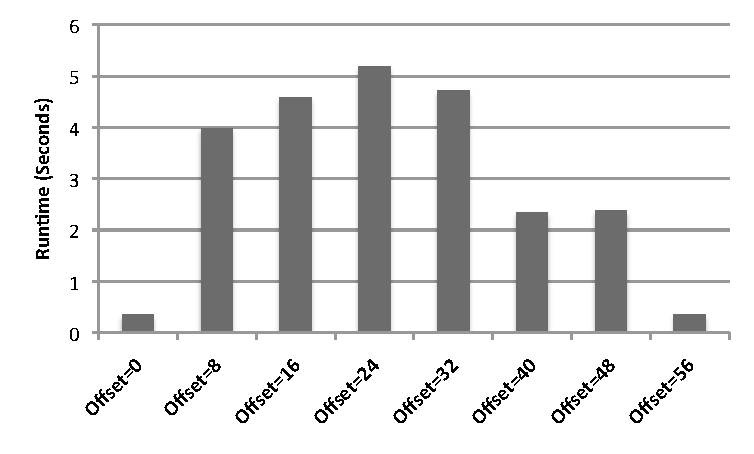
\includegraphics[width=3.3in]{fig/perfsensitive}
\end{center}
\caption{
Performance of the \texttt{linear\_regression} benchmark from the Phoenix benchmark suite.
Performance is highly sensitive to the offset of the starting address of the (potentially) falsely-shared object 
and the start of cache line. 
\label{fig:perfsensitive}}
\end{figure}

The appearance of false sharing depends on 
the alignment between objects and corresponding cache lines.
\CC{A real example, linear\_regression, is shown in Figure~ref{fig:perfsensitive}.}
For this benchmark,
when the offset of the starting address between the potentially falsely-shared object and corresponding cache lines 
is $0$ or $56$ bytes, 
there is no false sharing. 
When the offset is $24$ bytes, we see the most severe performance effect caused 
by false sharing. 
The performance difference between these two scenarios can be as large as $15\times$. 
Existing detection tools can only report observed false sharing.
For this case, they may miss a very severe false sharing problem that could occur in the wild if the offset of the starting 
address was $0$ bytes or $56$ bytes in their test environment.
\Predator{} overcomes this shortcoming by accurately predicting potential false sharing.

\begin{figure*}
\begin{center} 
\subfigure[No false sharing]{%
   \label{fig:nofs}
   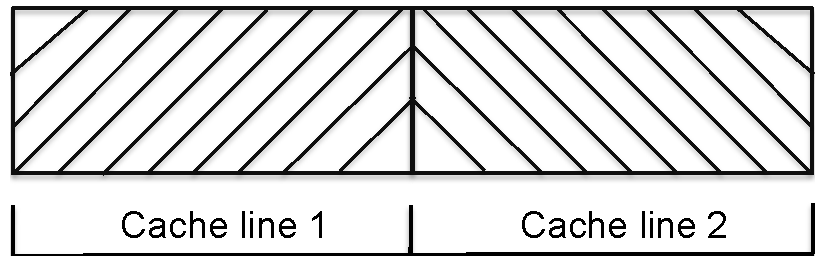
\includegraphics[width=0.24\textwidth]{fig/Potential1}
}%
\hspace{30pt}
\subfigure[False sharing with larger cache size]{%
   \label{fig:fslarger}
   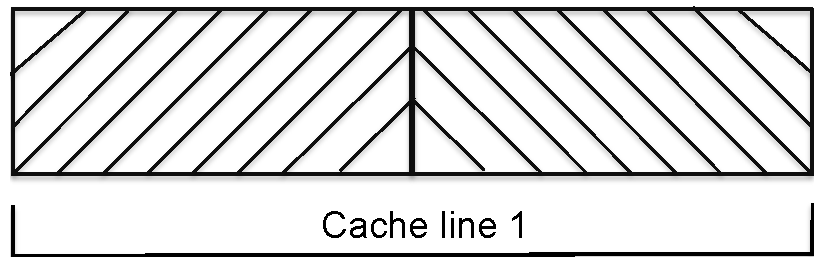
\includegraphics[width=0.24\textwidth]{fig/Potential2}
}%
\hspace{30pt}
\subfigure[False sharing with different alignment]{%
   \label{fig:fsnoalignment}
   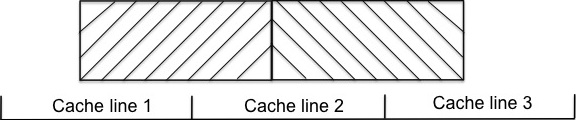
\includegraphics[width=0.36\textwidth]{fig/Potential3}
}%
\end{center}
%\includegraphics{fig/potential.pdf}
\caption{False sharing under different environments.}
\label{fig:potentialfalsesharing}
\end{figure*}

\Predator{} predicts {\it potential false sharing}, the type of
false sharing that does not 
manifest in the current execution but may appear and greatly affect programs' performance
in a slightly different environment.

Figure~\ref{fig:potentialfalsesharing} shows a simplified example why occurrences of false sharing 
can change in different situations.
In this figure, two rectangles with different patterns
represents two portions of the same object, updated by different threads. 
In Figure~\ref{fig:nofs}), there is no false sharing when thread T1 only updates 
``cache line 1'' and T2 only updates ``cache line 2''.
However, false sharing appears in one of the following cases, even with the same
access pattern. 

\begin{itemize}
\item
Doubling cache line size (Figure~\ref{fig:fslarger}). When the size of a
cache line doubles,
both T1 and T2 access the same cache line and false sharing occurs in this case.

\item
Different starting address of an object(Figure~\ref{fig:fsnoalignment}). 
When the starting address of this object is not aligned with the starting address of 
the first cache line, 
then T1 and T2 can update the second cache line simultaneously, 
causing false sharing. 
%When some dynamic property changes the starting address of this object so that it 
%is not aligned with the starting address of the first cache line, 
\end{itemize} 

\Predator{} predicts whether programs can have potential false sharing  
in either of these two cases, where they can be caused by different dynamic properties 
discussed in Section~\ref{sec:intro}.
All dynamic properties, except the change of cache line size,
can lead to different starting address of an object. 
Thus, predicting false sharing in these two cases actually 
explores many possibilities caused by all dynamic properties.

\subsection{Basic Prediction Workflow}
\label{sec:predictionmechanism} 

%Similar to the detection part, 
\Predator{} focuses exclusively on potential false sharing that can 
cause performance problems.
The implementation is based on
two key observations. First, only accesses to 
adjacent cache lines can form potential false sharing, 
i.e., introducing cache invalidations when cache line size
or an object's starting address changes.
Second, only when false sharing introduces a large number of cache invalidations
can it degrade performance.

Based on these two observations, \Predator{} develops 
the following workflow to capture potential false sharing.
Those detection optimizations listed in Section~\ref{optimization} can also be applied
to prediction part. We do not repeat these optimizations in this section.

\begin{enumerate}
\item
Track the number of writes on different cache lines. 

\item
When the number of writes to a cache line $L$ reaches {\it Tracking-Threshold},
track the detailed read and write accesses for every word on both cache line $L$ 
and its adjacent cache lines. 

\item
When the number of writes to a cache line $L$ reaches a second threshold (called as
{\it Predicting-Threshold}), 
identify whether there exists false sharing in $L$ and its adjacent 
cache lines by analyzing word accesses information collected in Step 2. 
Section ~\ref{sec:evaluatingfs} describes the evaluation method.

\item
If a potential false sharing is found, continue to track cache line invalidations to confirm it. Section~\ref{sec:tracking} discusses the details.
Otherwise, go back to Step 2 to track more detailed accesses.
 
\end{enumerate}

\subsection{Searching for Potential False Sharing}
\label{sec:evaluatingfs}
To describe potential false sharing in two different cases, we first 
introduce the concept of a virtual cache line.  A virtual cache line
is a contiguous memory range that spans one or more physical cache 
lines.  In the case of double cache line size, a virtual line is
composed of two original contiguous cache lines and the first cache
line has an even index number.  Thus, only cache lines $2*i$ and
$2*i+1$ can form a virtual line.  In the case of different starting
addresses, a virtual line can have the same size as physical lines,
but can be positioned arbitrarily: unlike actual cache lines, the
starting address of a virtual cache line does not need to be multiple
of the cache line size.  For instance, a 64-byte long virtual line can
consist of the range $[0,64)$ bytes or $[8,72)$ bytes.

To search for potential false sharing problems, 
\Predator{} searches for a hot access pair on $L$ and its adjacent cache lines 
by analyzing the detailed word access information collected in Step 2. 
A hot access in a cache line refers to the word whose number of read or write accesses 
is larger than the average number of accesses to each word of cache line $L$.
For every hot access $X$ in cache line $L$, \Predator{} searches another
hot access $Y$ in $L$'s previous cache line or next cache line satisfying
the following conditions: 

\begin{itemize}
\item
$X$ and $Y$ reside on the same virtual line. 

\item
One of $X$ and $Y$ is a write access.

\item 
$X$ and $Y$ are issued by different threads.

\end{itemize}

% why it finds a pair of $X$ and $Y$ == a potential false sharing 
Whenever it finds such a pair $X$ and $Y$, 
\Predator{} identifies potential performance-degrading false sharing whenever
 the number of cache invalidations caused by $X$ and $Y$, at a possible virtual line, 
is larger than the average number of accesses on each word of $L$. 
This approach is based on a similar observation as in detection:
\emph{if a thread writes a virtual line after other threads 
have accessed the same virtual line, this write operation most likely causes at least one cache 
invalidation}. 
\CC{
Before tracking detailed memory accesses on this cache line, it is impossible to know exactly how many cache invalidations happen on a virtual line. Thus, \Predator{} conservatively assumes that accesses from different threads are interleaved.
This approach ensures that \Predator{} does not miss any potential false sharing as well as 
not reporting false positives. }

%According to above observation and assumption, 
%a pair of hot accesses, $X$ and $Y$, if accesses are issued in an interleaving 
%way, can generate the number of cache invalidations equaling to 
%the smaller number of accesses of $X$ and $Y$.
%Thus a false sharing problem is to be identified by \Predator{}.
  
After identifying possible false sharing, \Predator{} goes to Step 4 to 
verify whether this is an actual false sharing problem.

\subsection{Verifying Potential False Sharing}
\label{sec:tracking}

\Predator{} verifies potential false sharing by tracking 
cache invalidations on a problematic virtual line.
%covering a pair of hot accesses found
%in Step 3.

For potential false sharing caused by double cache line size, as described in
Section~\ref{sec:evaluatingfs}, a virtual line is always composed of 
cache line with index $2*i$ and $2*i+1$. 
\Predator{} tracks cache invalidations
on the virtual line on which false sharing has been discovered.

However, for the case of a change in starting address,
two hot accesses with distance less than cache line size 
can form multiple virtual lines. 
There is thus an additional step to determine which virtual line to be tracked.
Although the virtual line to be chosen here is never a real cache line of actual hardware
because of unaligned addresses,
we utilize this virtual line to simulate the effect of changing the 
starting addresses of objects.


\begin{figure}
\begin{center} 
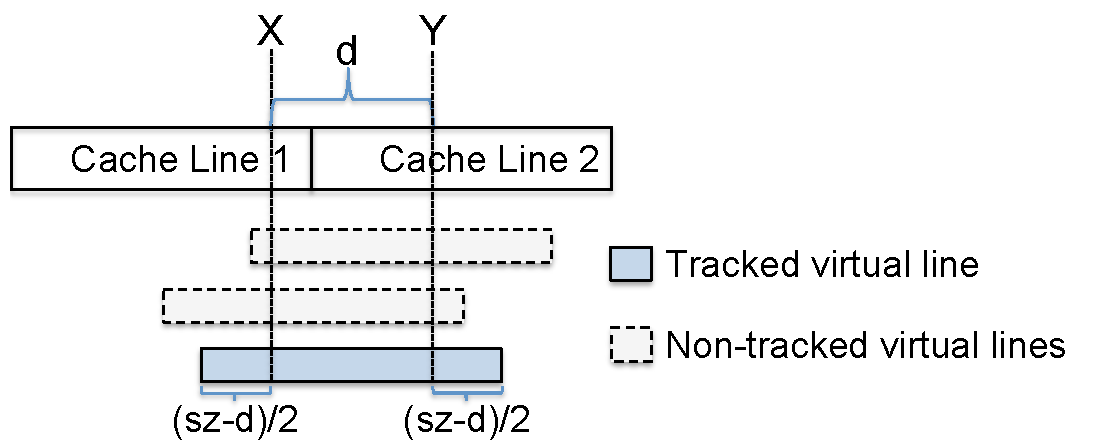
\includegraphics[width=3.3in]{fig/trackpotential}
\end{center}
\caption{Determining a virtual line with size $sz$ according to hot accesses.}
\label{fig:trackpotential}
\end{figure}

Given two words with the hot accesses shown in Figure~\ref{fig:trackpotential}, 
\Predator{} leaves the same space before $X$ and after $Y$ in determining a virtual line. 
That is, the virtual line starting 
at location $X-((sz-d)/2)$ and ending at $Y+((sz-d)/2)$ is tracked. 
This choice allows tracking of more possible cache invalidations caused by
adjacent accesses of $X$ and $Y$. 
Since adjusting the starting address of a virtual line has the same effect of
adjusting the starting address of an object in detecting false sharing,
all cache lines related to the same object must be adjusted at the same time.
\Predator{} then tracks cache invalidations based on these adjusted virtual lines.

\subsection{Reporting Potential False Sharing}
Reporting potential false sharing problems shares the same mechanisms and optimizations 
used in detection. These are discussed in Section~\ref{sec:runtime}.


%\input{Prediction}

\section{Experimental Evaluation}
\label{sec:evaluation}

All evaluations are performed on a quiescent Intel Core 2 dual-processor system equipped with 
16GB of RAM. 
%whereas each processor has 4 cores. 
%processor with 4 cores), with 8GB of RAM. 
Each processor is a 4-core 64-bit Intel Xeon running at 2.33 GHz with a 4MB
shared L2 cache and 32KB private L1 cache. 
The underlying operating system is unmodified CentOS 5.5, running with Linux kernel
version 2.6.18-194.17.1.el5. The glibc version is 2.5. 
In order to compare the performance fairly, all benchmarks were built as 64-bit executables 
using LLVM compiler (version 3.2). The compiler optimization level is set to ``-O1'' 
so memory allocation callsites can be reported precisely.
%since we can not report line number of source code with optimization level larger than
%``-O2''.
In our evaluation, we choose two popular benchmark suites, Phoenix~\cite{phoenix-hpca} and PARSEC~\cite{parsec}.

Our evaluations aim to answer the following questions:
\begin{itemize}
\item
  How effective is \defaults{} on detecting and predicting false sharing problem (Section ~\ref{sec:effective})?

\item
  What is the performance overhead of \defaults{} with and without prediction
  (Section ~\ref{sec:perfoverhead})?

\item
  What is the memory overhead of \defaults{}~ (Section~\ref{sec:memoverhead})?
\end{itemize}


\subsection{Detection and Prediction Effectiveness}
\label{sec:effective}

\subsubsection{Benchmarks}
To compare with state-of-the-art false sharing detection work~\cite{sheriff, OSdetection}, 
we also executes \defaults{} on two existing benchmark suites 
suites Phoenix~\cite{phoenix-hpca} and PARSEC~\cite{parsec}, 
and results are listed in the Table~\ref{table:detection}. 

%Our results show that \defaults{} not only capture previously-discovered
%false sharing, but also many detect new false sharing places. The results
%are listed in Table~\ref{table:detection}. 

%http://www.technovelty.org/tips/getting-a-tick-in-latex.html
%http://tex.stackexchange.com/questions/42619/x-mark-to-match-checkmark
%\begin{comment}
\begin{table*}[ht!]
{
\centering
\begin{tabular}{l|r|r|r}
\hline
{\bf \small Benchmark} & {\bf \small Source Code} & {\bf \small New} & {\bf \small Improvement} \\
%{\bf \small Benchmark} & {\bf \small Source Code} & {\bf \small Type of False Sharing} & {New} & {\bf \small Improvement} \\
\hline
\small \textbf{histogram} & {\small histogram-pthread.c:213} & \cmark{} & 46.22\%\\
\small \textbf{reverse\_index} & {\small reverseindex-pthread.c:511} & \xmark{} & 0.09\%\\
\small \textbf{word\_count} & {\small word\_count-pthread.c:136} & \xmark{} & 0.14\%\\
\hline
\small \textbf{streamcluster} & {\small streamcluster.cpp:985} & \xmark{} & 7.52\% \\
\small \textbf{streamcluster} & {\small streamcluster.cpp:1907} & \cmark{} & 4.77\%\\
%\small \textbf{bodytrack} & {\small TrackingModel.cpp:59} & 0 & \cmark{} & \\
\hline
\hline
\small \textbf{linear\_regression} & {\small linear\_regression-pthread.c:133} & \xmark{} & 1206.93\%\\
\hline
\end{tabular}
\caption{Detection results of \defaults{} on Phoenix and PARSEC benchmark suites. \label{table:detection}}
}
\end{table*}

In this table, the first column lists those programs with false sharing problems. 
The second column shows precisely where the problem is. Actually, all false sharing found
are internal object false sharing on heap objects, although \defaults{} has no 
problem to find intern-objects and global false sharing. So the memory allocation site 
are listed in the table.
The third column ``New'' marks whether this false sharing is newly found by \defaults{} or not.
False sharing found by previous work are marked as cross mark(\xmark{}) and those 
newly found false sharing are identified using a tick mark(\cmark{}). 
The last column ``Improvement'' shows the performance improvement after fixing false sharing 
based on the average result with $10$ runs. 
The improvement rate is calculated by substracting $1$ from normalized runtime. Taking 
\texttt{histogram} for an example here, original runtime of \texttt{histogram} is $0.75s$
and new runtime is $0.51s$, then the performance improvement is $(0.75/0.51) - 1$.

Seen from the table, \defaults{} reveals several unknown false sharing problems. \defaults{} detects 
false sharing in \texttt{histogram} and additional false sharing in line 1908 of
\texttt{streamcluster}. 
In \texttt{histogram}, multiple threads repeatedly modify different locations of the same heap object. 
Padding the data structure \texttt{thread\_arg\_t} fixes the false sharing problem and 
helps to improve the performance around 46\%.
In \texttt{streamcluster}, multiple threads are changing a \texttt{bool} array, \texttt{switch\_membership}, simultaneously. By simply changing this array to \texttt{long} type contributes to about 4.7\% performance improvement. 
%None of these two false sharing problems has been reported by previous tools.

Other false sharing problems has been revealed by previous tool \sheriff{}~\cite{sheriff}. 
Same as \sheriff{}, we didn't see much performance improvement for \texttt{reverse\_index} and 
\texttt{word\_count} since number of updates inside them is not a significant number. But they
are actually false sharing problems that have been verified manually by us.

\texttt{streamcluster} has another false sharing problem that different threads 
may change the same object simultaneously. 
Actually authors of \texttt{streamclsuter} have already realized possible
false shairing problems and meant to utilize a macro \texttt{CACHE\_LINE} to avoid it. Unfortunately,
the defaulted value of this macro is setted to $32$ bytes, which is different with the actual
cache line size that we are using. By setting to $64$ bytes instead, we see around $7.5\%$ performance
improvement.

linear\_regression has a significant false sharing problem. 
Different threads simultaneously changed an array of thread-indexed structures in a tight
loop, which causes a huge amount of cache invalidations. 
Fixing false sharing inside can improve the performance for $12\times$. 
Actually, if we do not enable prediction then 
we can not detect false sharing problem inside because false sharing behavior is 
very sensitive to the starting address of false sharing object. 
We are going to explore this more detailed in Section~\ref{sec:predicteval}.
Since \defaults{} are using a customized memory manager, which may
bring us different allocation metadata and different memory map for allocation,
false sharing problem may not manifest with ``-O1'' optmization flag of \texttt{clang}.
%http://tex.stackexchange.com/questions/42619/x-mark-to-match-checkmark
%\begin{comment}

\subsubsection{Real Applications}
To verify its practicability, we further evaluate \defaults{} 
on several widely-used real applications, which none of previous work has considered.  
These real applications include a server application \texttt{MySQL}~\cite{mysql}, 
a common C++ library \texttt{boost}~\cite{libfalsesharing} 
and a distributed memory object caching system \texttt{memcached}, a network retriver \texttt{aget}, 
a parallel bzip2 file compressor \texttt{pbzip2} and a parallel file scanner \texttt{pfscan}.
Among them, \texttt{MySQL} and \texttt{boost} are known to have some false sharing problem inside 
so we evaluate their specific versions, \texttt{MySQL-5.5.32} and
\texttt{boost-1.49.0}.

False sharing in \texttt{MySQL} has caused significant scalability problem and
it was very difficult to be identified. 
According to the architect of \texttt{MySQL} Mikael Ronstrom, ``we had gathered specialists on 
InnoDB..., participants from MySQL support... and a number of generic specialists on 
computer performance...'', ''the fruit of the meeting ... were able to 
improve \texttt{MySQL} performance by 6$\times$ with those scalability fixes''. 
The false sharing of boost library is caused by the special usage of \texttt{spinlock} pool and fixing
it brings 40\% performance improvement. 
\defaults{} is able to succesfully detect false sharing locations
in \texttt{MySQL} and \texttt{boost} library. 
For the other four applications, \defaults{} doest not find serere false sharing problems.

\subsubsection{Prediction Effectiveness}
\label{sec:predicteval}
We evaluates the prediction effectiveness of \defaults{} on the \texttt{linear\_regression} benchmark.
We choose this benchmark for two reasons:
\begin{enumerate}
\item
False sharing problem of this benchmark can not be detected without prediction. 

\item
This benchmark has a severe performance problem when false sharing actually occurs, which should be 
detected but can be omitted by exiting tools.
\end{enumerate}

The data structure of false sharing object and the source code
to experience false sharing is showed in Figure~\ref{fig:linearregression}. 
When we are using \texttt{clang} compiler while compiling for $64$bit binary, the size of this 
data structure is $64$ bytes.

\begin{figure}[!h]
{\centering
\subfigure{\lstinputlisting[numbers=none,frame=none,boxpos=t]{fig/linearregression.psedocode}}
\caption{False sharing problem inside \texttt{linear\_regression} benchmark.
\label{fig:linearregression}}
}
\end{figure}

For this false sharing problem, the main thread allocates an array of $8$ elements 
(if $8$ cores totally), 
with each element being a \texttt{lreg\_args} type. 
Then this array will be passed to different threads so that they can only updates its 
thread-dependent area, see Figure~\ref{fig:linearregression}.
Actually, different fields of this data structure \texttt{lreg\_args} has different access pattern:
only those fields between $SX$ and $SXY$ (totally around $40$ bytes) are constantly read and updated.

Thus, \texttt{linear\_regression} actually is very sensitive to the starting address 
of the false sharing object, which can be caused by many of dynamic properties 
listed in Section~\ref{sec:intro}, e.g.,
hardware platform, optimization flag, compiler etc.
This sensitivity can be seen in Figure~\ref{fig:perfsensitive}.
That is, when offset is $0$ or $56$ bytes, there is no false sharing at all.
Actually, using our customized memory manager,
the offset between the starting address of potential false sharing object 
and starting of cache line is actually $56$ bytes,
that explain why we can not detect false sharing problem without prediction enabled.

\defaults{} can predict false sharing problem precisely for all of these cases. This explains
the effectiveness of prediction tool.

\subsection{Performance Overhead}
\label{sec:perfoverhead}
To avoid the effect caused by extreme outliers,
all performance data are based on the average of 10 runs excluding the
maximum and minimum values.
Actual performance overhead can be seen in the following figure~\ref{fig:perf}. 

\begin{figure*}[!ht]
\begin{center}
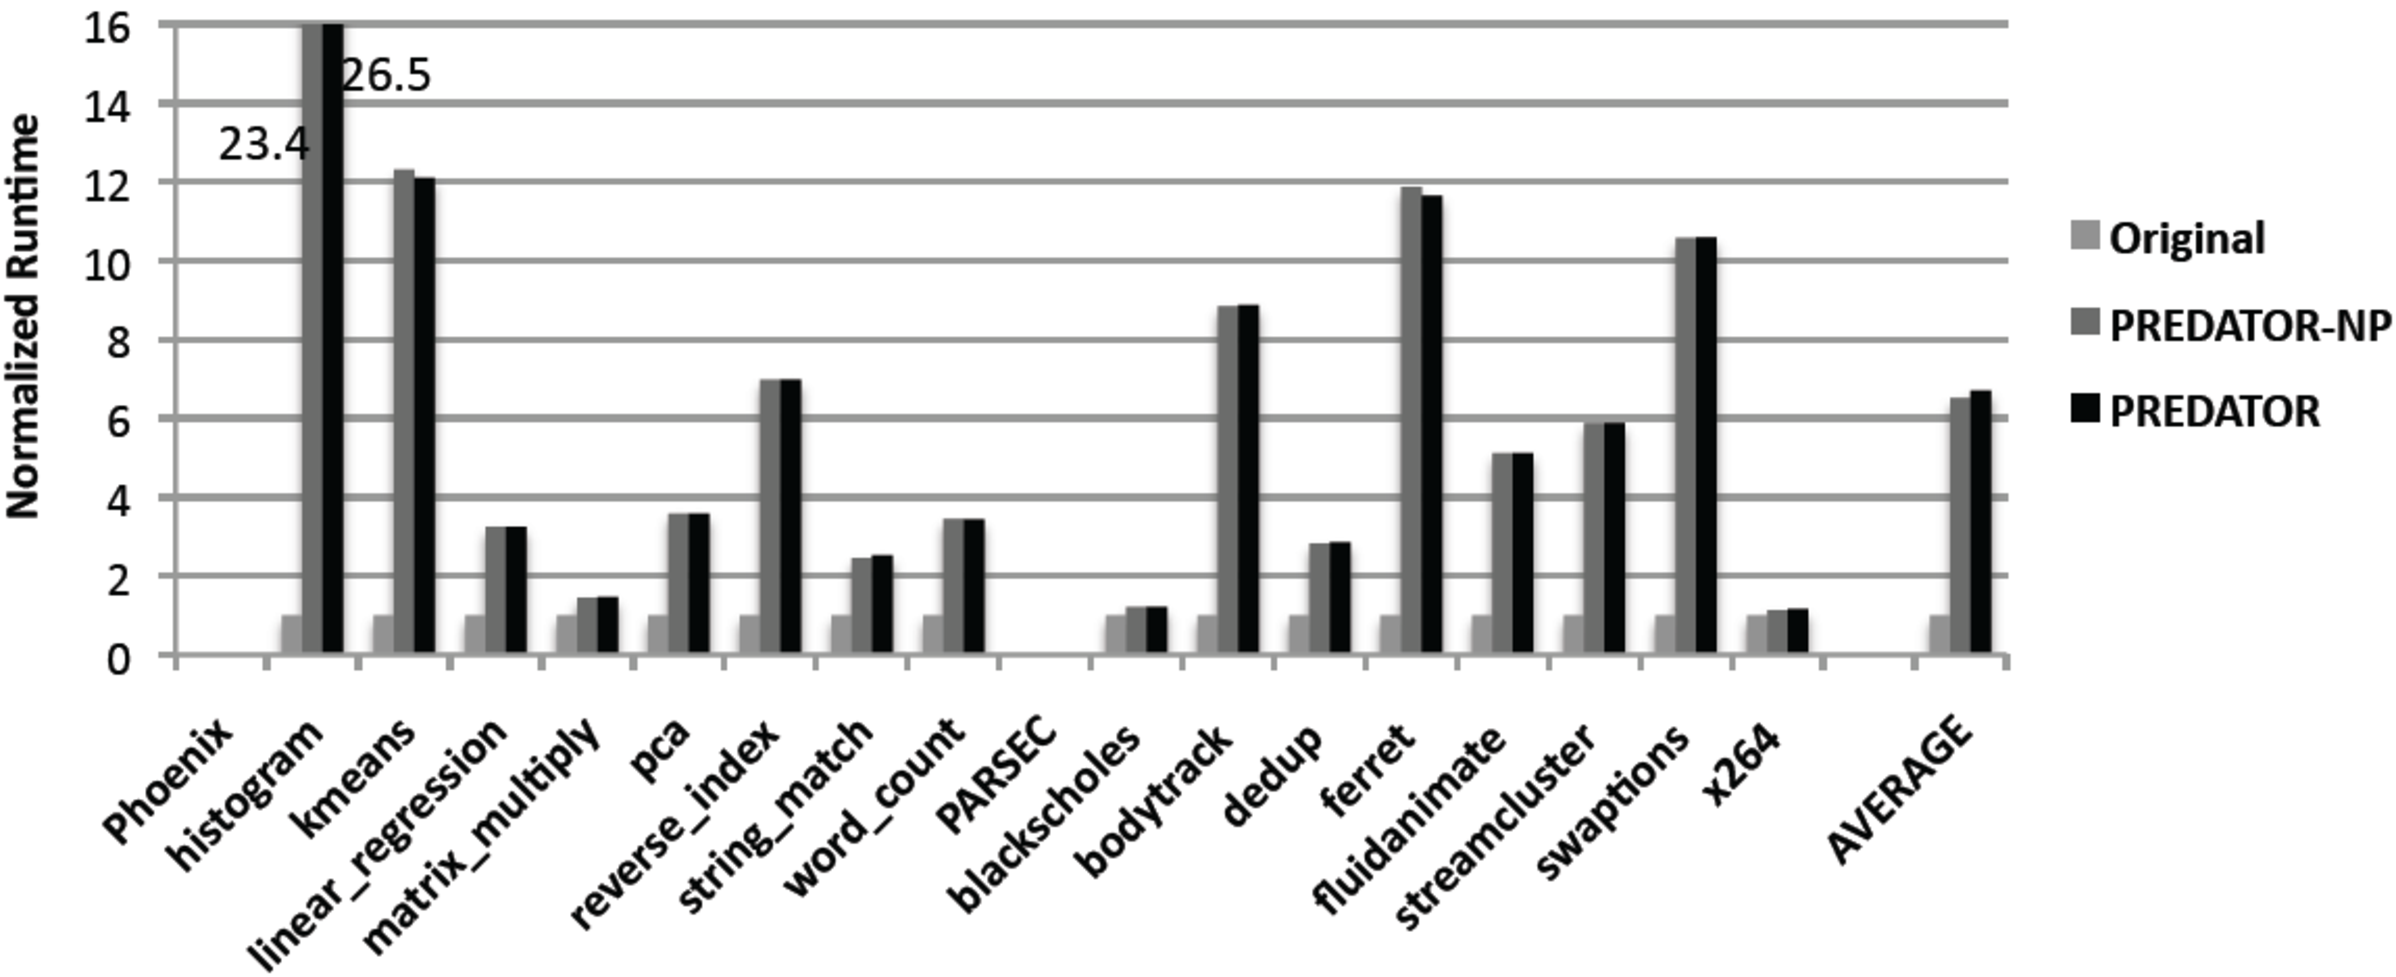
\includegraphics[width=5in]{fig/perf}
\end{center}
\caption{
Performance overhead of \defaults{} with and without prediction.
\label{fig:perf}}
\end{figure*}

Manifestness of false sharing highly depends on 

\subsection{Memory Overhead}
\label{sec:memoverhead}
Since \defaults{} pre-allocates a huge block of memory using \texttt{mmap} system call for 
its heap usage, 
virtual memory can not be used to tell actual memory overhead imposed by our tool. 
Hence, we only evaluate the physical memory overhead used by an application only. 
This number is based on proportional set size (PSS) in \texttt{/proc/self/smaps}
as discussed by Justin et al. ~\cite{memusage}. 

When evaluating an application, we start a script program to save 
corresponding \texttt{smaps} files periodically. 
The maximum number of total physical memory usage is selected for calculation.
%It is noted that we remove the physical memory usage of   
Results of memory usage is shown in Figure~\ref{fig:memusage}. As we can see,
\defaults{} does not increase memory usage substantially in all cases except for \texttt{swaptions}. 
Specifically, removing \texttt{swaptions} from calculation reduces 
the average memory overhead from 64\% to 22\%. 

The reason of \texttt{swaptions} using a large amount of memory is that 
its original memory usage is too small (only 3KB), and 
the additional memory added by \defaults{} in detection, prediction and
reporting yields a large number in percentage calculation. 

\begin{figure*}
\begin{center} 
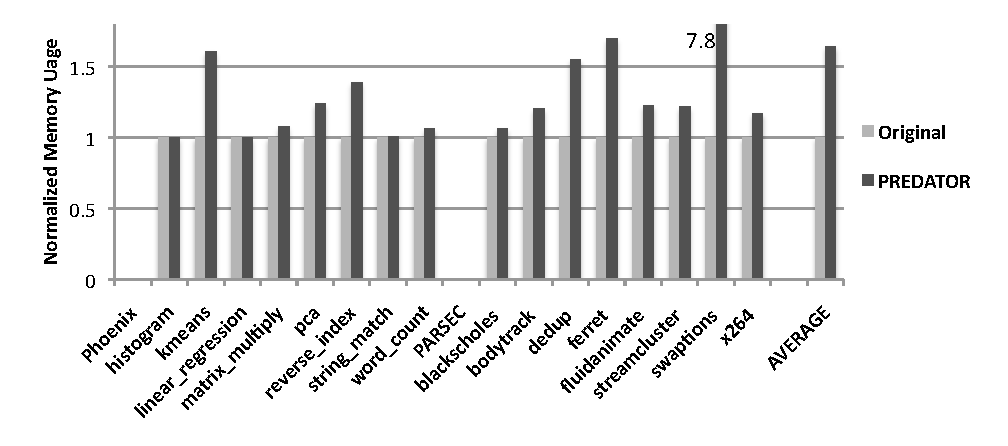
\includegraphics[width=5in]{fig/memusage}
\end{center}
%\includegraphics{fig/potential.pdf}
\caption{Memory usage overhead}
\label{fig:memusage}
\end{figure*}




\section{Discussion}
\label{sec:discussion}

\subsection{Instrumentation Selection}
\label{sec:instrumentationtradeoff}
Dynamic instrumentation and compiler instrumentation are two different approaches for instrumentation~\cite{Instrumentation}. They have different tradeoffs on performance and versatility. Dynamic instrumentation approaces normally analyze the program's code before the execution in order to insert instrumentation, such as Valgrind ~\cite{Valgrind}, Pin~\cite{Pin}, and DynamoRIO~\cite{DynamoRIO}. They introduce significant performance overhead, mostly caused by run-time encoding and decoding, but provide better versatility because of no recompilation. Compiler instrumentation inserts instrumentation in the compilation phase, which needs the source code to rebuilt, with less versatility. 
Compiler instrumentation is chosen here because of its better performance (~\cite{Instrumentation}) and more flexible instrumentation(discussed in Section~\ref{sec:selectinstrumentation}). For performance reason, \Predator{} can instrument or skip specific code or data. For example, the user could provide a black list so that given modules, functions or variables are not instrumented. Conversely, the user could provide a white list so that only specified functions or variables are instrumented.

\subsection{Important Factors}
The effect of sampling rate has been evaluated in Section~\ref{sec:sensitivity}.  We discuss several other important factors here. 

\paragraph{Input} Different inputs can cause different executions of a program. If a specific input does not exercise the code with false sharing problems, \Predator{} definitely cannot detect those false sharing problems. It shares the same attribute as that of all dynamic tools. However, \Predator{} can generalize over inputs to find latent false sharing problems on those exercised code. When any reasonably representative set of inputs are exercised, as is required by any testing regime, \Predator{} will be effective to detect false sharing.

\paragraph{Input Size} Input size may affect detection results.  As discussed in Section~\ref{optimization}, \Predator{} introduces several threshold values to reduce the tracking overhead, which can be adjusted based on actual detection environment. If input is so small that it cannot generate enough false sharing events to pass predefined thresholds,  then the detection mechanism may not be triggered. Thus, \Predator{} can miss certain false sharing problems. However, fair large input size should be enough to trigger our detection mechanism. Actually, all evaluated applications take less than 150 seconds to expose false sharing problems inside. 

\paragraph{Memory Hierarchy} Memory hierarchy of the underlying experimental machine cannot affect \Predator{}'s detection results. \Predator{} conservatively assumes that different threads are running on different cores and detects false sharing problems basing on possible cache invalidations. \Predator{} does not acquire the actual cache invalidations of a program, which can be affected by real memory hierarchy of the underlying experimental machine. Thus, \Predator{} does not bind to a specific machine, providing better generality than tools using hardware performance counters. A deeper hierarchy should only amplify the costs of false sharing, and thus exemplify the value of \Predator{}.

\subsection{Prediction Limitation} 
\Predator{} can accurately and precisely predict false sharing problems without the need of occurrence. But \Predator{} cannot  predict a false sharing problem if the code with false sharing inside is not exercised at all. Also, \Predator{} may miss potential inter-objects false sharing problems caused by using different compilers or memory allocators. 

\section{Future Work}
\label{sec:future}
\label{futurework}

We plan to extend \sheriff{} to find more performance related problems in
multithreaded programs. For example, if one frequently-read word
happens to be in the same cache line with one frequently-written word,
it would be better to separate those two words. But in the current
framework, \sheriff{} cannot detect a single memory read operation using the
twin page mechanism. We are examining the combination of hardware
watchpoints to help us locate this kind of performance error. In
addition, we plan to exploit watchpoints to capture those program
counters that touch specific addresses so as to point the programmer
to specific lines of code responsible for false sharing.




%\section{Issues}
%(1) Maybe user should have a option to check those false sharing inside stack variables.
(2) Should we use a thread index instead to save some spaces? Also, maybe it is better for the performance. 
    Generally, we will not have two threads that are accessing the same subheap. However, we may have to use
    the pthread\_t for comparison since it is unique? but actually it is not.
    We should use the unique heap in order to avoid the lock usage and overlapping (Diehard problem). In Diehard,
    two threads can use the same heap every time. 
    Also, we may introduce the current pointer in the thread library so that we can know corresponding information quickly. 
    whenever all children threads has been exited, then we should possibly update the 
    So we should use a

(3) Should we have an internal heap which also use tid to index their subheap.
(4) When there are multiple files there, how we can instrument every file one by one? Design a makefile to do this automatically. 

(a) Inserting the into clang so that we do not need to change the make file for each files.
(b) We will keep track of each read/write accesses instead of only checking once for each basic block.


Improving the performance step by step
(1) Avoiding using the singleton if we can use the simple variable.
(2) Trying to use the sampling (100 instructions we only sample one).

(4) How to sample those accesses. We donot want to loose those cache invalidations. 
So for each cache line, we are using the cache line based sampling mechanism. 
In the non-sampling phase, we will not update everything. 

However, there is a per-thread based sampling. For example, we only sample those accesses in the 
first 500 over 1000 accesses. However, we may lost a lot of interleaving accesses by doing this. 

If we are using the system level accessCount, for example, updating this shared accesses can cause a lot of
invalidations - which cause a lot of performance problem by using the shared account.

Also, we should try to implement those very basic accesses incremental in the first level instead of inside a very deep level.



\section{Related Work}
\label{sec:relatedwork}

This section describes related work in false sharing detection, prevention, or both; no prior work predicts false sharing.

\subsection{False Sharing Detection}
Schindewolf et al.\ designed a tool based on the SIMICS functional simulator to report different kinds of cache usage information, such as cache misses and cache invalidations~\cite{falseshare:simulator}. Pluto relies on the Valgrind dynamic instrumentation framework to track the sequence of memory read and write events on different threads, and reports a worst-case estimation of possible false sharing~\cite{falseshare:binaryinstrumentation1}.
Similarly, Liu uses Pin to collect memory access information, and reports total cache miss information~\cite{falseshare:binaryinstrumentation2}.
These tools impose about $100-200\times$ performance overhead.

Zhao et al.\ present a tool based on the DynamoRIO framework to detect false sharing and other cache contention problems
for multithreading programs~\cite{qinzhaodetection}. 
It uses a shadow memory technique to maintain memory access history and detects cache invalidations based on the ownership of cache lines. However, it can only support at most $8$ threads. In addition, it cannot differentiate cold cache misses from actual false sharing problems.

Intel's performance tuning utility (PTU) uses Precise Event Based Sampling (PEBS) hardware support to detect false sharing problems~\cite{detect:ptu,detect:intel}.  PTU cannot distinguish true sharing from false sharing. In addition, PTU aggregates memory accesses without considering memory reuse and access interleavings, leading to numerous false positives. Sanath et al.\ designed a machine learning based approach to detect false sharing problems. They train their classifier on mini-programs and apply this classifier to general programs~\cite{mldetect}. Instead of instrumenting memory accesses, this tool relies on hardware performance counters to collect memory accesses events. This approach operates with extremely low overhead but ties false sharing detection to a specific hardware platform.

In addition to their individual disadvantages,
all approaches discussed above share a common shortcoming:  
they cannot pinpoint the exact location of false sharing in the source code, so programmers must manually examine the source code to identify problems.

Pesterev et al.\ present DProf, a tool that help programmers identify cache misses based on AMD's instruction-based sampling hardware~\cite{DProf}. DProf requires manual annotation to locate data types and object fields, and cannot detect false sharing when multiple objects reside on the same cache line.

\subsection{False Sharing Prevention}

Jeremiassen and Eggers use a compiler transformation to automatically adjust the memory layout of applications through padding and alignment~cite{falseshare:compile}. Chow et al.\ alter parallel loop scheduling in order to avoid false
sharing~\cite{falseshare:schedule}. These approaches only works for regular, array-based scientific code.

Berger et al.\ describe Hoard, a scalable memory allocator that can reduce the possibility of false sharing by making different threads use different heaps~\cite{Hoard}. Hoard cannot avoid false sharing problem in global variables or within a single heap object: the latter appears to be the primary source of false sharing problems.

\subsection{False Sharing Detection and Prevention}

\sheriff{} provides two tools to handle false sharing based on its ``threads-as-processes'' framework~\cite{sheriff}.
\Sheriff{}'s detection tool reports false sharing accurately and precisely with only $20\%$ performance overhead.
However, it can only detect write-write false sharing, and only works for programs that use the \pthreads{} library. It can also break programs that communicate across different threads with stack variables or \emph{ad hoc} synchronizations. These shortcomings limit \Sheriff{}'s usefulness for real-world applications.  
\Predator{} can detect all kinds of false sharing and imposes no limitations on the kind of applications it works on. 

\Sheriff{}'s prevention tool prevents false sharing altogether, eliminating the need for programmer intervention. However, in programs with many synchronization calls, the overhead imposed by \Sheriff{} could lead to performance degradation.

Plastic leverages the sub-page granularity memory remapping facility provided by the Xen hypervisor to detect and tolerate false sharing automatically~\cite{OSdetection}. However, the sub-page memory remapping mechanism is not currently supported by most existing operating systems, reducing its generality. In addition, Plastic cannot pinpoint the exact source of false sharing.  
In order to utilize Plastic's prevention tool, a program has to run on the Xen hypervisor, limiting the applicability of their prevention technique.


\section{Conclusion}
This paper introduces \emph{evidence-based dynamic analysis}, a new
lightweight dynamic analysis technique. Evidence-based dynamic
analysis works for errors that can be forced to leave evidence of
their presence. These errors include key problems for C and C++
programs: buffer overflows, dangling-pointer errors, and memory
leaks. Evidence-based dynamic analysis is fast because it lets the
application run at full speed until an error is detected; execution is
then rolled back and replayed with instrumentation at the point where
the evidence was found, pinpointing the error. We
present \doubletake{}, the first evidence-based dynamic analysis
framework, and implement these analyses inside it. The resulting
analyses are the fastest versions to date, demonstrating the
effectiveness and efficiency of this new dynamic analysis approach.
\doubletake{} is available for download at \url{http://github.com/plasma-umass/DoubleTake}.



\section{Acknowledgement}
The authors thank Junjie Gu for his help on LLVM. 
We also thank Charlie Curtsinger, John Alditor and anonymous reviewers for their precious suggestions which helped improve this paper. Most implementation of this work are conducted when Tongping was interning in Huawei 
US research center. \CC{We also acknowledge the support of NSF****** }.  


%\appendix
%\section{Manual}

%\section{How to Integrate with LLVM}





% We recommend abbrvnat bibliography style.

%\bibliographystyle{abbrvnat}

% The bibliography should be embedded for final submission.
{
\bibliographystyle{abbrv}
\bibliography{refs}
}

%\begin{thebibliography}{}
%\end{thebibliography}

\end{document}
